\documentclass[preprint,12pt,authoryear]{elsarticle}

\usepackage{amsmath,amssymb}
\usepackage{booktabs}
\usepackage{threeparttable}
\usepackage{tabularx}
\usepackage{longtable}
\usepackage{graphicx}
\usepackage{siunitx}
\usepackage{microtype}
\usepackage{enumitem}
\usepackage{xurl}
\usepackage{hyperref}
\usepackage{cleveref}

\hypersetup{
  colorlinks=true,
  linkcolor=black,
  citecolor=black,
  urlcolor=blue
}

\graphicspath{{../outputs/eda/delu_features/development/development_a03fix_v1/figures/}}

\journal{Energy Economics}

\newcommand{\EUR}[1]{€#1}

\begin{document}

\begin{frontmatter}

\title{Forecast-to-Trade under Information Constraints: Frozen Out-of-Sample Evidence from the Germany--Luxembourg Day-Ahead Electricity Market}

\author[knust]{Jonathan Nelson\corref{cor1}}
\ead{jonathannelson707@gmail.com}
\cortext[cor1]{Corresponding author.}
\address[knust]{Kwame Nkrumah University of Science and Technology (KNUST), Kumasi, Ghana}

\begin{abstract}
Electricity-price forecasts are commonly judged by statistical errors even though their operational value depends on the decisions they support. This study evaluates whether a forecasting advantage survives point-in-time information constraints and translates into economic value under a frozen out-of-sample protocol for the Germany--Luxembourg day-ahead market. Public ENTSO-E data from 2019--2025 are used for development, while January--July 2026 is reserved for a first-look holdout. The information set is split into a Full specification and a Tier-1 robustness specification that excludes wind- and solar-derived variables whose exact historical availability at the simulated 11:45 D-1 decision time cannot be verified. XGBoost is selected during development against naive and ElasticNet benchmarks, and uncertainty is estimated from delivery-day-safe empirical residual quantiles. Forecasts are then mapped into a pre-specified single-cycle storage decision rule with a frozen efficiency--cost sensitivity grid. On 5,087 holdout hours, Full XGBoost attains an MAE of \EUR{17.51}/MWh versus \EUR{29.33}/MWh for lag-24. Under the primary economic assumptions, the Full point strategy earns \EUR{20,002.02} compared with \EUR{18,564.42} for lag-24, and the incremental value remains positive in all nine pre-specified sensitivity cells. The uncertainty-aware Full strategy sacrifices \EUR{872.01} of aggregate P\&L but raises the trade hit rate from 91.9\% to 99.4\% and improves the worst day from \EUR{-17.55} to \EUR{-0.83}. Tier-1 remains superior to lag-24 but materially weaker than Full. The contribution is therefore methodological and evidential rather than algorithmic: forecast value is assessed under explicit information-timing boundaries, delivery-day-safe uncertainty, frozen pre-exposure rules, economic robustness and tail-risk diagnostics.
\end{abstract}

\begin{keyword}
electricity price forecasting \sep Germany--Luxembourg \sep XGBoost \sep battery arbitrage \sep forecast uncertainty \sep economic value \sep out-of-sample evaluation
\end{keyword}

\end{frontmatter}

\section{Introduction}
\label{sec:introduction}

Electricity price forecasting occupies an unusual position in forecasting research. Forecast errors are statistically measurable, but the practical value of reducing them depends on the decisions made with the forecasts. This distinction is especially important in day-ahead electricity markets, where prices can be negative, exhibit abrupt spikes, and respond nonlinearly to load, renewable generation and market conditions. These features have motivated a large literature spanning autoregressive models, regularized regression, machine learning and probabilistic forecasting \citep{weron2014,zielweron2018,lago2021}. Yet improvement in a conventional accuracy measure such as mean absolute error (MAE) is not, by itself, evidence that a forecast produces a better economic decision.

The distinction between statistical and economic forecast quality is established prior work. \citet{kathziel2018} explicitly connect electricity-price forecast quality to realized economic gains, while \citet{serafin2025} show that choices affecting forecast loss can materially alter both trading profit and risk. Most recently, \citet{maciejowska2026} compare 192 forecasting specifications in the German/Germany--Luxembourg market and show that RMSE and MAE are only weakly related to battery-arbitrage income. The same issue extends to probabilistic forecasts: \citet{nitka2023} find that a statistically better predictive-distribution combination need not generate higher realized profit. The relevant research question is therefore not whether accuracy and economic value can diverge, but whether a forecasting advantage remains useful when the information set, uncertainty method and economic decision rule are all constrained ex ante.

That requirement is more demanding than it appears. A day-ahead forecasting exercise is economically meaningful only if each predictor could have been available when the simulated decision was made. Historical electricity databases often contain load, wind, solar and other variables that are highly informative ex post. Their presence in a historical API, however, does not establish that the particular stored value was publicly available at the relevant forecast origin. Publication deadlines, revisions and data vintages therefore matter. Prior work supports the predictive usefulness of fundamentals and weather information \citep{kathziel2018,sgarlato2023}, but that evidence does not prove that every historical ENTSO-E renewable forecast used in a new application was available at a specific pre-auction timestamp.

A second difficulty concerns evaluation design. Electricity-price models are typically developed through repeated choices over features, algorithms, hyperparameters, calibration windows and error measures. Unless these choices are separated from the final evaluation period, reported out-of-sample performance can become contaminated by iterative model development. The best-practice literature therefore emphasizes chronological testing, strong benchmarks, common evaluation samples and model selection that does not use the final test period \citep{weron2014,lago2021}. This discipline is even more important when forecasts feed an economic strategy, because thresholds, costs, uncertainty filters and operating rules can themselves be tuned after observing profits.

This study addresses these issues through an end-to-end forecast-to-decision experiment for the Germany--Luxembourg (DE-LU) day-ahead electricity market. The empirical sample starts on 1 January 2019, after the German--Austrian bidding-zone split. The simulated forecast and decision origin is fixed at 11:45 Europe/Berlin on D-1. Public ENTSO-E price and fundamental data are cleaned under explicit local-delivery-day logic, including daylight-saving-time transitions and the move of Single Day-Ahead Coupling (SDAC) to 15-minute market time units for delivery from 1 October 2025 \citep{entsoe2025}.

The predictor set is divided into two information levels. The \emph{Full} specification contains lagged prices, calendar effects, the day-ahead load forecast, renewable-generation forecasts and variables derived from them. The \emph{Tier-1} specification removes the wind- and solar-derived variables whose precise historical public availability at 11:45 D-1 cannot be established from the historical ENTSO-E interface. This distinction does not assert that those variables contain look-ahead information. It identifies an evidential boundary: their exact vintage at the simulated forecast origin is not reconstructable from the data source used here.

All model development is restricted to 2019--2025. Naive 24-hour and 168-hour lags provide transparent benchmarks, ElasticNet provides a regularized linear benchmark, and XGBoost is evaluated as a nonlinear challenger. Model selection is chronological. Forecast uncertainty is estimated from out-of-sample residuals and corrected to respect the common whole-day D-1 forecast origin: every hour of delivery day \(D\) uses residual information from delivery dates strictly earlier than \(D\). Because the selected residual offsets are common to all hours within a delivery day, the resulting uncertainty-aware economic rule is algebraically a day-varying abstention threshold rather than an alternative intraday pair-selection rule.

Economic value is evaluated with a deliberately transparent storage-arbitrage rule rather than a full battery-dispatch model. Each day allows at most one charge interval and one later discharge interval. Six strategies distinguish no trading, lag-based decisions, Full and Tier-1 XGBoost decisions, and uncertainty-filtered variants. Before the holdout is opened, the primary efficiency and degradation assumptions, the entire \(3\times3\) sensitivity grid, the uncertainty procedure and the primary economic confirmation rule are frozen.

The final evaluation uses a first-look holdout from 1 January through 31 July 2026. Its structural completeness was checked before outcome exposure, but its realized prices were not used for model selection, tuning, uncertainty-window choice, strategy design or economic interpretation. The final forecasting models, uncertainty method and economic rules were frozen before the first 2026 performance metric was inspected.

The holdout produces three central findings. First, Full XGBoost retains a large predictive advantage: MAE is \EUR{17.51}/MWh compared with \EUR{29.33}/MWh for lag-24 and \EUR{24.36}/MWh for Tier-1 XGBoost. Second, the forecasting improvement translates into economic value under the pre-specified decision rule. At the primary parameter setting, the Full XGBoost point strategy earns \EUR{20,002.02} versus \EUR{18,564.42} for lag-24, and the incremental value remains positive in all nine pre-specified efficiency--cost cells. Third, uncertainty filtering is not unambiguously profit-enhancing. The Full uncertainty-aware strategy gives up \EUR{872.01} of cumulative net P\&L but increases the trade hit rate from 91.9\% to 99.4\% and improves the worst daily result from \EUR{-17.55} to \EUR{-0.83}.

The contribution is consequently methodological and evidential rather than algorithmic. The paper combines: (i) an explicit point-in-time information boundary through Full and Tier-1 specifications; (ii) a pre-specified protocol frozen before holdout exposure; (iii) a genuine first-look 2026 holdout; (iv) a pre-specified nine-cell economic robustness criterion; (v) delivery-day-safe uncertainty implemented transparently as an abstention threshold; and (vi) economic and tail-risk diagnostics. The study does not claim that XGBoost is universally superior, that lower MAE necessarily implies greater economic value, or that the stylized storage results constitute deployable investment returns.

The remainder of the paper is organized as follows. Section~\ref{sec:literature} positions the study in the forecasting, uncertainty and storage-value literature. Section~\ref{sec:data} describes the market, data and information-set construction. Section~\ref{sec:methods} presents forecasting, uncertainty and economic methods. Section~\ref{sec:development} reports development evidence and the freeze decisions. Section~\ref{sec:holdout} presents the frozen 2026 holdout. Section~\ref{sec:discussion} discusses interpretation and limitations, and Section~\ref{sec:conclusion} concludes.

\section{Literature review and research positioning}
\label{sec:literature}

\subsection{Electricity price forecasting and credible comparison}

Electricity price forecasting has developed from relatively compact time-series models into a broad field containing high-dimensional regression, machine learning, deep learning and probabilistic methods. The expansion reflects the unusual behavior of wholesale electricity prices: strong seasonal structure, spikes, negative prices and sensitivity to system fundamentals and market design \citep{weron2014}. The resulting empirical literature provides little support for assuming that one model class will dominate across all markets and periods. In a large multi-market comparison, \citet{zielweron2018} find that model structure and predictor choice matter materially and that no universal winner emerges between high-dimensional univariate and multivariate frameworks.

The machine-learning literature has enlarged the set of credible models rather than removed the need for careful comparison. \citet{lagodeep2018} demonstrate strong performance from deep-learning approaches in a broad benchmark, while \citet{lago2021} emphasize that claims of model superiority are meaningful only when evaluation is based on transparent data, strong baselines, chronological testing and uncontaminated model selection. Their open benchmark and associated \texttt{epftoolbox} provide an important reproducibility reference for the present study.

These lessons shape our forecasting design. Lag-24 and lag-168 forecasts are retained as simple market-aware baselines; ElasticNet represents a regularized linear benchmark; and XGBoost enters as a challenger rather than being presumed superior. The model choice is therefore an empirical result of the development sample, not the paper's novelty claim.

\subsection{Fundamentals and the information available at the forecast origin}

Electricity prices respond to expected system conditions, making load and renewable-generation forecasts natural predictors. High-dimensional German electricity-price models have long incorporated wind, solar and calendar information \citep{ziel2015}, while \citet{kathziel2018} use public load and renewable fundamentals in quarter-hourly German forecasting. Weather predictions also contain useful price information at longer horizons \citep{sgarlato2023}.

However, predictive usefulness and point-in-time availability are distinct. Historical databases frequently store a final or revised forecast series without preserving every publication vintage. A variable that is observable to the researcher today is not automatically one that would have been observable at the simulated decision time.

This distinction is central to the present study. Regulation (EU) No 543/2013 requires day-ahead load forecasts to be published no later than two hours before the relevant day-ahead gate closure, whereas day-ahead wind and solar generation forecasts are required no later than 18:00 Brussels time on D-1 \citep{eureg543}. With the regular SDAC order book closing at 12:00 \citep{epex2025}, the regulatory deadline for load is compatible with an 11:45 cutoff, while the renewable deadline is not. The historical API also does not expose the complete publication-vintage history required to establish the exact timestamp of the stored renewable forecast. Our Full/Tier-1 design therefore makes the uncertainty around information availability visible rather than assuming it away.

\subsection{From forecast accuracy to economic value}

Forecasts acquire operational value through the decisions they change. Storage arbitrage provides a natural test because its value depends on identifying low-price and high-price intervals. Foundational storage studies establish the economic importance of temporal price spreads and the sensitivity of value to efficiency and operating assumptions \citep{sioshansi2009}. More recent European evidence documents substantial day-ahead arbitrage opportunities across markets \citep{mercier2023}. Yet perfect-foresight storage optimization is an upper bound rather than a test of a real forecasting system.

The distinction between perfect and forecast-based information has therefore become increasingly important. \citet{sharma2021} review forecasting in energy-storage applications and caution against operational conclusions based only on perfect or artificial forecasts. \citet{prakash2025} similarly show that the quality of future pricing information materially influences storage scheduling value.

\citet{kathziel2018} provide a particularly close conceptual predecessor by explicitly quantifying the economic gains from more accurate German electricity-price forecasts. Their work establishes that forecast improvements can produce measurable economic value, but also that the decision rule matters. More recently, \citet{serafin2025} show that forecasting loss functions can change both profits and risk, and that costs and trading frequency affect economic rankings.

The closest contemporary comparator is \citet{maciejowska2026}. Using 192 forecast specifications for the German/Germany--Luxembourg day-ahead market, they show that MAE and RMSE are only weakly associated with BESS profits and that measures capturing intraday shape and extrema can be more economically informative. This evidence makes an important novelty boundary explicit: the proposition that lower statistical error need not imply higher storage value is established prior art. Our contribution lies instead in testing forecast value under a frozen point-in-time information and economic protocol.

\subsection{Probabilistic forecasting and decision quality}

Point forecasts suppress uncertainty that may be highly relevant in a volatile electricity market. Probabilistic electricity-price forecasting therefore evaluates both calibration and sharpness \citep{nowotarski2018}. Regularized quantile regression averaging can improve the robustness of probabilistic forecasts and can support profitable decisions in some settings \citep{uniejewskiweron2021}. Modern distributional neural networks likewise connect probabilistic performance with economically relevant forecast evaluation \citep{marcjasz2023}. These approaches sit within the broader theory of proper scoring rules, where the statistical objective is to reward honest predictive distributions \citep{gneiting2007}.

Better statistical uncertainty, however, does not guarantee better decisions. \citet{nitka2023} show that a CRPS-optimized combination of predictive electricity-price distributions can be statistically more accurate without generating higher trading profit than a simpler aggregation scheme. This result parallels the point-forecast literature and motivates evaluating our uncertainty layer through its actual decision consequences rather than assuming that improved interval behavior must increase P\&L.

The present uncertainty method is deliberately simple: rolling empirical residual quantiles are applied to the selected point forecasts. The methodological emphasis is not a new probabilistic model but information-set discipline. The entire delivery day is decided at D-1 11:45; consequently, no realized residual from day \(D\) may influence any uncertainty bound for day \(D\). This day-origin restriction distinguishes the final implementation from ordinary sequential hourly rolling intervals.

\subsection{Research gap}

The literature establishes that EPF is market-specific, that fundamentals can add predictive value, that accuracy and economic value can diverge, and that probabilistic improvements may or may not enhance realized decisions. It also establishes that costs, efficiency and trading frequency matter for economic evaluation \citep{serafin2025,maciejowska2026}.

The gap addressed here concerns how these strands are combined under a single pre-exposure research design. First, the historical information boundary is explicit through Full and Tier-1 information sets. Second, model selection, uncertainty selection and the economic strategy are frozen before final outcome exposure. Third, the primary economic conclusion must survive a pre-specified nine-cell efficiency--cost grid rather than one favorable operating assumption. Fourth, uncertainty is constructed at the same whole-day information origin as the decision problem. Finally, profit, abstention, downside, oracle value capture and empirical tail risk are reported jointly.

The resulting contribution is therefore not a new forecasting architecture. It is a controlled forecast-to-trade experiment that asks a narrower question with stronger evidential discipline: does a forecasting improvement developed on public market data survive an untouched period, remain economically useful under pre-specified operating assumptions, and how does that conclusion change when information restrictions and uncertainty are imposed?

\section{Market setting, data and information set}
\label{sec:data}

\subsection{Germany--Luxembourg day-ahead market}

The empirical application focuses on the Germany--Luxembourg (DE-LU) day-ahead bidding zone. The sample begins on 1 January 2019, after the German--Austrian bidding-zone split, and all market logic is defined by Europe/Berlin delivery dates. UTC is used internally for storage and joins.

The simulated analyst forms the complete delivery-day forecast at 11:45 Europe/Berlin on D-1. This is before the regular SDAC order-book gate closure at 12:00 \citep{epex2025}. From delivery day 1 October 2025, SDAC moved from hourly to 15-minute market time units \citep{entsoe2025}. The forecasting and economic system remains hourly throughout: pre-cutover hourly prices enter directly, while post-cutover quarter-hourly prices are averaged within each hour. A regime indicator marks observations after the transition.

\subsection{ENTSO-E data}

Three data categories are retrieved from the ENTSO-E Transparency Platform:

\begin{table}[htbp]
\centering
\caption{ENTSO-E variables used in the study.}
\label{tab:data_sources}
\begin{adjustbox}{max width=\textwidth}
\begin{tabular}{llll}
\toprule
Component & Document type & Unit & Role \\
\midrule
Day-ahead price & A44 & EUR/MWh & Target and lagged prices \\
Day-ahead total load forecast & A65 & MW & Tier-1 fundamental \\
Day-ahead wind/solar forecast & A69 & MW & Tier-2 renewable inputs \\
\bottomrule
\end{tabular}
\end{adjustbox}
\end{table}

Raw XML responses are cached using request parameters, while ingestion metadata preserve retrieval timestamps, requested windows, data types and row counts. This makes the processed feature set traceable to the raw ENTSO-E responses used in the analysis.

The complete processed feature file contains 66,455 hourly observations. The 2019--2025 development period contains 61,368 rows, while the 2026 holdout contributes 5,087 common point-evaluation rows across 212 delivery days.

\subsection{Price reconstruction and market-product selection}

A44 retrievals require explicit market-product selection. The historical ENTSO-E response contains parallel products that can share timestamps but differ in resolution. The production series retains the hourly product before the 15-minute SDAC transition and the 15-minute product thereafter.

A second ambiguity arises from \texttt{classificationSequence}. The final production series retains sequence 1. This choice was externally audited against SMARD: among 8,833 corrected-data intervals in which sequences 1 and 2 differed materially, the SMARD price matched sequence 1 in every case and sequence 2 in none. The audit therefore supports sequence 1 as the continuing reference series used in this study.

The XML parser also reconstructs ENTSO-E \texttt{curveType=A03} correctly. Under A03, only positions where the value changes need to be reported explicitly; intervening values inherit the previous block value. An earlier parser version treated such positions as missing. The corrected parser reconstructs the complete period before aggregation, and all results in this paper use the corrected \texttt{a03fix} lineage.

\subsection{Time normalization and daylight-saving time}

All raw timestamps are converted to timezone-aware UTC. Local delivery dates, hours, days of week and months are then derived using Europe/Berlin conversion. Market-design boundaries are defined by local delivery day rather than UTC midnight. This is necessary because the delivery day 1 October 2025 begins at 22:00 UTC on 30 September 2025 while summer time is in force.

Load, wind and solar forecasts are reported at quarter-hourly resolution throughout the sample and are therefore averaged to hourly MW values over the full history. Price aggregation is conditional on the market-design cutover because the primary day-ahead price product itself changes resolution at that date.

The three data sources are outer-joined by UTC timestamp so that a missing fundamental remains visible rather than causing the price row to disappear.

\subsection{Fundamental and historical-price features}

Aggregate forecast renewable generation is
\begin{equation}
\widehat R_t=
\widehat W_t^{on}+\widehat W_t^{off}+\widehat S_t,
\end{equation}
residual load is
\begin{equation}
\widehat{RL}_t=\widehat L_t-\widehat R_t,
\end{equation}
and renewable share is
\begin{equation}
\widehat{RS}_t=\frac{\widehat R_t}{\widehat L_t},
\end{equation}
for positive load forecasts.

Missing wind components are not treated as zero. Both onshore and offshore wind must be present before aggregate wind is formed. Solar missingness observed during development is concentrated in non-generating nighttime intervals and is treated as zero only for construction of the aggregate renewable variables.

Historical price state is represented by 24-, 48- and 168-hour lags and rolling mean and volatility features over 24-hour and 168-hour windows. The hourly grid is regularized before lagging so that a row displacement remains an actual time displacement even when the raw series contains gaps.

A fixed 24-hour UTC lag is not always sufficient on a 25-hour autumn DST day to guarantee that the source value belongs to an earlier local calendar date. The pipeline therefore invalidates any lagged observation that cannot be proven to cross the local delivery-date boundary. Rolling statistics inherit the same restriction.

Calendar features include cyclic sine and cosine representations of hour, day of week and month, a weekend indicator, weekend--hour interactions, and the post-15-minute-MTU regime indicator.

\begin{figure}[htbp]
\centering
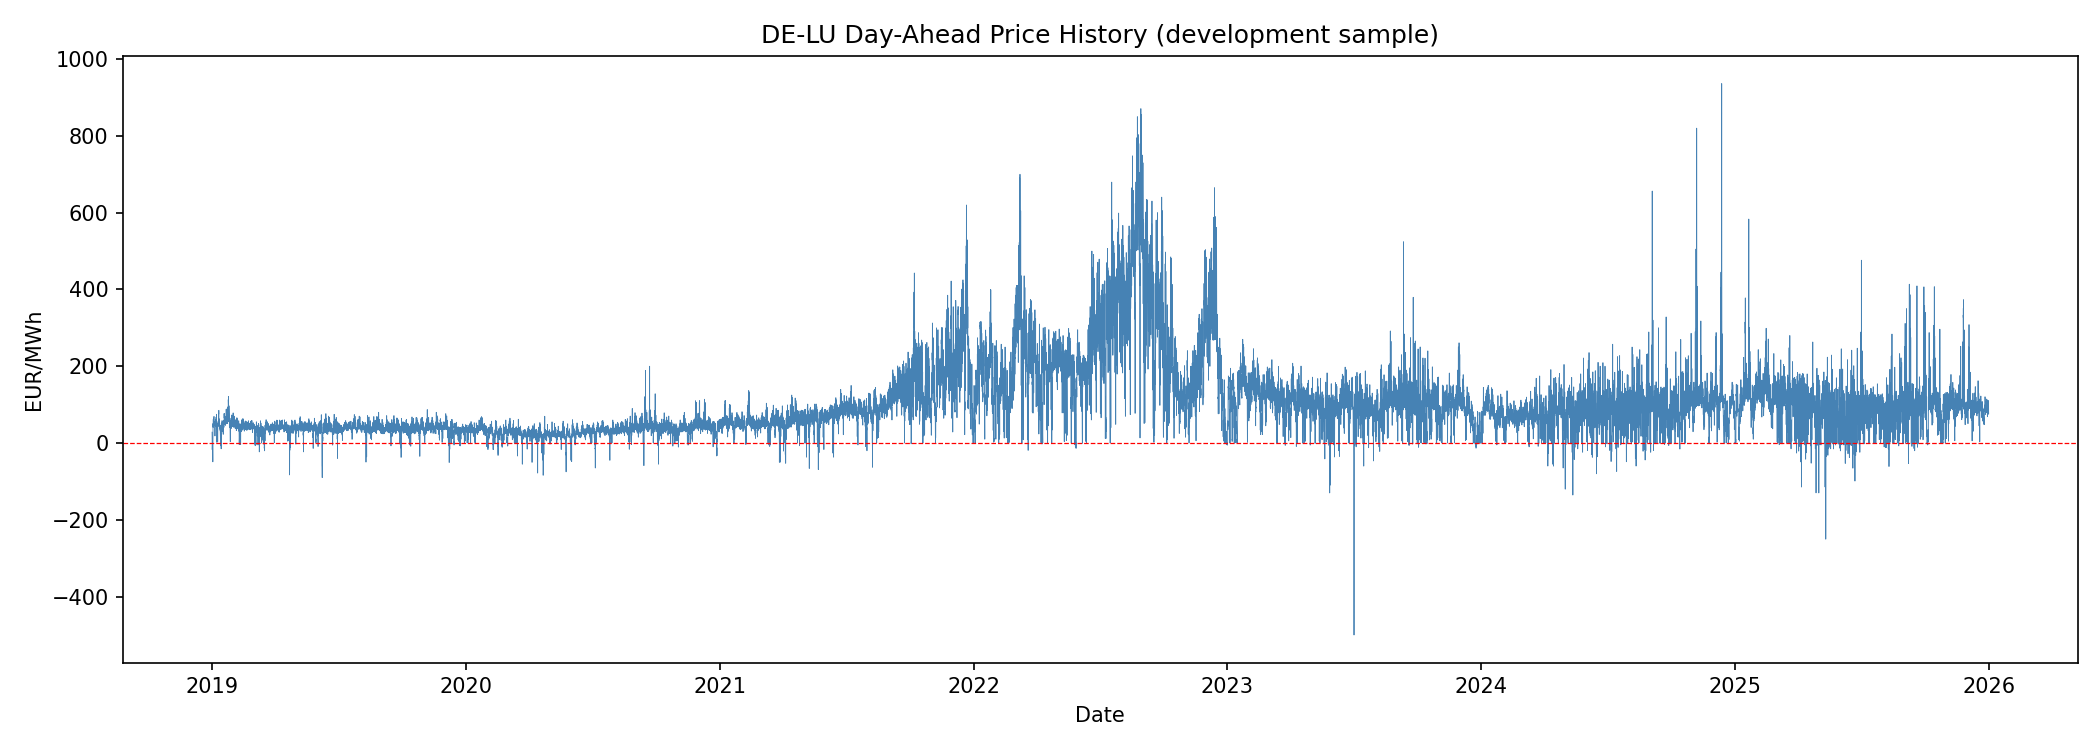
\includegraphics[width=\linewidth]{fig1_price_history.png}
\caption{DE-LU day-ahead hourly price history in the development sample.}
\label{fig:price_history}
\end{figure}

\begin{figure}[htbp]
\centering
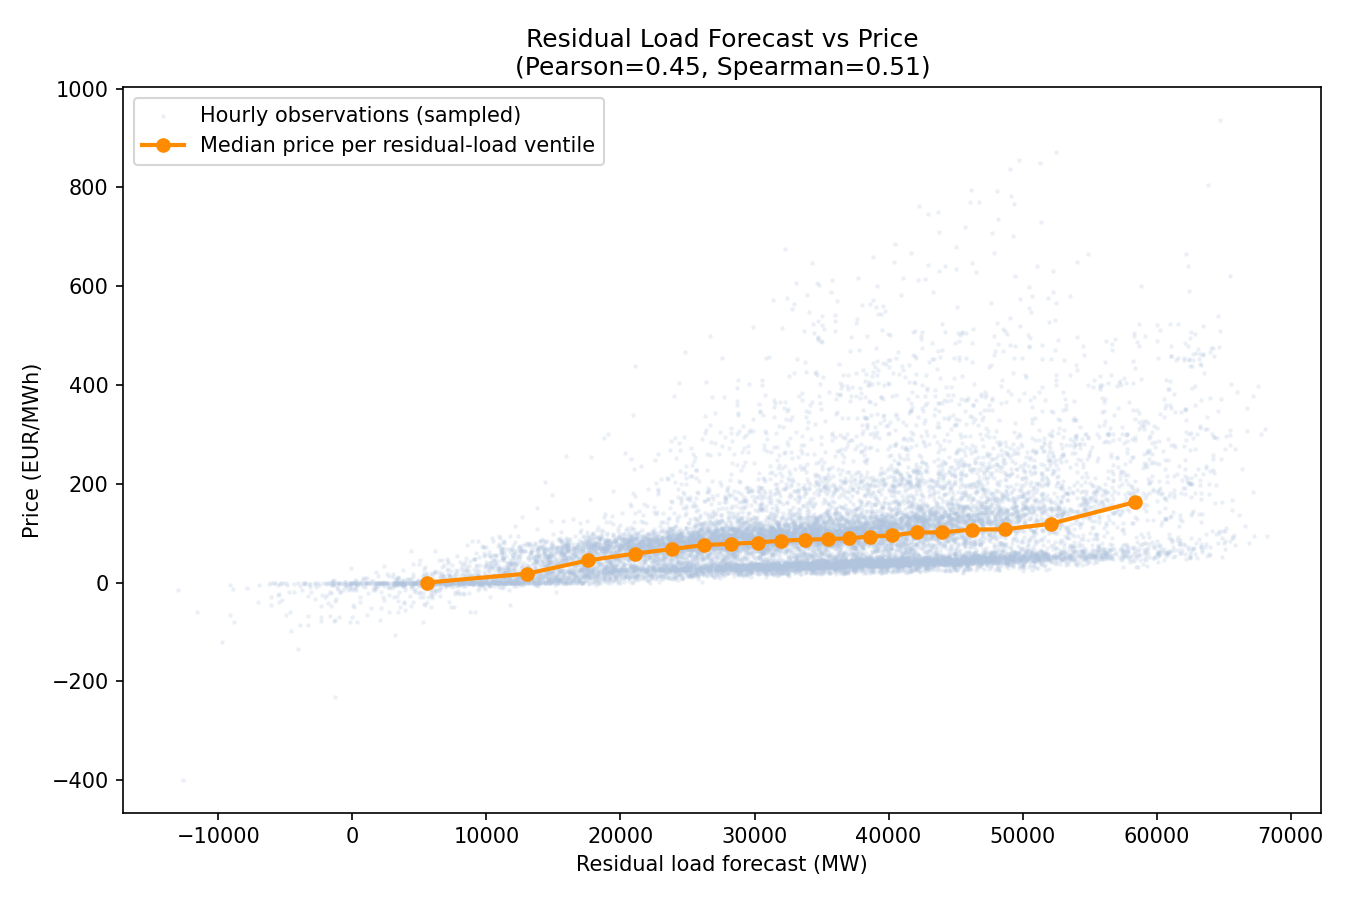
\includegraphics[width=0.85\linewidth]{fig4_residual_load_vs_price.png}
\caption{Development-sample relationship between forecast residual load and day-ahead price.}
\label{fig:residual_load}
\end{figure}

\subsection{Point-in-time information tiers}

The central information-set distinction follows the simulated 11:45 D-1 forecast origin. Regulation (EU) No 543/2013 requires day-ahead total load forecasts no later than two hours before the relevant day-ahead gate closure \citep{eureg543}. This regulatory deadline is compatible with the 11:45 cutoff, although exact historical revision vintages remain unreconstructed.

The same regulation requires day-ahead wind and solar generation forecasts no later than 18:00 Brussels time on D-1, with subsequent intraday updates \citep{eureg543}. That deadline is after the simulated cutoff. Moreover, the historical interface used here does not provide the complete vintage history needed to establish whether the stored renewable forecast for each day existed at 11:45.

Accordingly, the \emph{Full} information set contains load plus aggregate renewables, residual load and renewable share, while the \emph{Tier-1} information set removes the three renewable-derived predictors. Tier-2 does not mean that a variable is proven to leak future information; it means that its exact point-in-time availability cannot be established from the available historical record.

The Full predictor vector contains 21 variables and Tier-1 contains 18. The Tier-1 comparison therefore asks how much predictive and economic performance survives when the unresolved renewable-vintage information is removed.

\subsection{Development and holdout separation}

Four chronological outer validation blocks are defined within development:

\begin{table}[htbp]
\centering
\caption{Chronological development splits.}
\label{tab:splits}
\begin{adjustbox}{max width=\textwidth}
\begin{tabular}{lll}
\toprule
Fold & Training period & Validation period \\
\midrule
1 & 2019--2022 & 2023 \\
2 & 2019--2023 & 2024 \\
3 & 2019--2024 & Jan--Sep 2025 \\
Regime stress & 2019--Sep 2025 & Oct--Dec 2025 \\
\bottomrule
\end{tabular}
\end{adjustbox}
\end{table}

No shuffling is permitted. After development decisions are frozen, the final Full and Tier-1 models are independently refitted on all eligible observations through 31 December 2025.

The final holdout is fixed as 1 January 2026 inclusive to 1 August 2026 exclusive. Structural checks of data presence, coverage and interval continuity were permitted before exposure, but 2026 outcome values were not used for model selection, uncertainty selection, strategy design or economic interpretation before the protocol was frozen.

\section{Methodology}
\label{sec:methods}

\subsection{Empirical design and forecast metrics}

The analysis proceeds through four layers: point forecasting, forecast uncertainty, economic decision-making and tail-risk evaluation. Development choices are completed before the 2026 holdout is opened.

The naive benchmarks are
\begin{equation}
\widehat P^{(24)}_t=P_{t-24}
\end{equation}
and
\begin{equation}
\widehat P^{(168)}_t=P_{t-168}.
\end{equation}

Point forecasts are evaluated using MAE, RMSE and median absolute error. MAE is the primary model-selection criterion:
\begin{equation}
MAE=\frac{1}{N}\sum_{t=1}^{N}|P_t-\widehat P_t|.
\end{equation}
Percentage-error measures are not used because electricity prices can be zero or negative.

Every model within an outer fold is evaluated on an identical common-row set. Stress diagnostics additionally examine negative prices and realized prices above \EUR{200}/MWh and \EUR{500}/MWh.

\subsection{ElasticNet benchmark}

ElasticNet provides the regularized linear benchmark. Predictors are standardized within a pipeline, ensuring that scaling is refitted inside each inner training fold. The accepted benchmark uses four-fold chronological hourly \texttt{TimeSeriesSplit} cross-validation, MAE scoring, 15 logarithmically spaced \(\alpha\) values from \(10^{-3}\) to \(10^2\), and
\[
\rho\in\{0.1,0.5,0.9,1.0\}.
\]
This procedure was frozen before the later XGBoost design and was not retrospectively altered after the delivery-day inner-CV issue described below was recognized.

\subsection{XGBoost model and day-aligned tuning}

XGBoost uses the same Full and Tier-1 predictor sets as ElasticNet. The estimator uses the absolute-error objective, histogram tree construction and random seed 42. The pre-specified grid is
\[
\text{max depth}\in\{3,4,5\},
\]
\[
\text{n estimators}\in\{200,400\},
\]
\[
\text{learning rate}\in\{0.03,0.05,0.10\},
\]
and
\[
\text{subsample}\in\{0.8,1.0\},
\]
giving 36 configurations.

XGBoost hyperparameters are selected using three chronological inner folds over unique Europe/Berlin \emph{delivery dates}. This keeps all 23, 24 or 25 observations of a local delivery day on the same side of an inner train-validation boundary. The choice matches the economic forecast origin: all prices for day \(D\) are formed together at D-1 11:45, so realized targets from the early hours of \(D\) should not influence model selection for later hours of that same day.

The development promotion rule required Full XGBoost to improve on the frozen Full ElasticNet pipeline by more than 1\% in row-weighted outer-fold MAE. The rule was specified before the first real-data XGBoost result.

\subsection{Final refit}

Once the development procedure was complete, Full and Tier-1 XGBoost were refitted independently on all development data. Each information set reran the same frozen 36-configuration search; hyperparameters were not transferred from one information set to the other.

The selected final configurations were:

\begin{table}[htbp]
\centering
\caption{Frozen final XGBoost configurations.}
\label{tab:final_hyperparams}
\begin{adjustbox}{max width=\textwidth}
\begin{tabular}{lrrrrr}
\toprule
Information set & Learning rate & Depth & Trees & Subsample & Rows \\
\midrule
Full & 0.10 & 3 & 200 & 0.80 & 61,142 \\
Tier-1 & 0.03 & 3 & 400 & 0.80 & 61,143 \\
\bottomrule
\end{tabular}
\end{adjustbox}
\end{table}

Model files, predictor lists and manifests were checksum-verified before holdout evaluation.

\subsection{Delivery-day-safe empirical uncertainty}

Uncertainty is constructed from genuinely out-of-sample development residuals,
\begin{equation}
e_t=P_t-\widehat P_t.
\end{equation}
The outer-fold XGBoost predictions from 2023--2025 form a continuous walk-forward residual history.

For delivery day \(D\), only residuals from delivery dates strictly before \(D\) are eligible. The empirical residual quantile is
\begin{equation}
r_D(q)=Q_q\left(\{e_t: D-w\leq delivery\_date(t)<D\}\right),
\end{equation}
and the corresponding hourly price quantile is
\begin{equation}
\widehat Q_{D,h}(q)=\widehat P_{D,h}+r_D(q).
\end{equation}

The frozen quantiles are \(q\in\{0.10,0.50,0.90\}\). Thus the nominal central 80\% interval is
\begin{equation}
[L_{D,h},U_{D,h}]
=
[\widehat Q_{D,h}(0.10),\widehat Q_{D,h}(0.90)].
\end{equation}

Candidate residual windows are \(w\in\{60,90,120,180,365\}\) delivery days. Each requires at least
\[
\max(1,\lfloor w/4\rfloor)
\]
days of history. Candidates are evaluated on one common observation set using the Winkler interval score. With \(\alpha=0.20\),
\begin{align}
IS_\alpha(L,U;P)
&=(U-L)
+\frac{2}{\alpha}(L-P)\mathbf{1}(P<L) \nonumber\\
&\quad+\frac{2}{\alpha}(P-U)\mathbf{1}(P>U).
\end{align}
Lower is better. The window with the lowest common-row score is selected mechanically; coverage diagnostics cannot override that result.

\subsection{Economic decision rule}

The economic layer is a stylized single-cycle daily storage problem. For each delivery day, all pairs \((i,j)\) satisfying \(i<j\) are candidates. A normalized one-unit charge is made at \(i\), with round-trip efficiency \(\eta_{rt}\) applied to the discharge leg.

Throughput degradation cost is
\begin{equation}
C_{deg}=c(1+\eta_{rt}),
\end{equation}
and market transaction cost is frozen at
\[
C_{market}=0.
\]
Total cost is
\begin{equation}
C=C_{deg}+C_{market}.
\end{equation}

For a point forecast, the decision score is
\begin{equation}
Score_P(i,j)=\eta_{rt}\widehat P_j-\widehat P_i-C.
\end{equation}
The strategy selects the highest-scoring pair and abstains if the best score is non-positive.

After the pair is fixed, realized net P\&L is
\begin{equation}
\Pi_D=\eta_{rt}P_{D,j^*}-P_{D,i^*}-C.
\end{equation}
Realized prices therefore value a decision already made from forecasts; they never select the trade.

For uncertainty-aware strategies, the conservative score is
\begin{equation}
Score_U(i,j)=\eta_{rt}L_j-U_i-C.
\end{equation}
This is a decision filter based on marginal bounds, not a jointly calibrated interval for the price spread.

The frozen strategies are:
\begin{description}[leftmargin=1.2cm,style=nextline]
\item[S0] no trade;
\item[S1] lag-24 point forecast;
\item[S2] XGBoost Full point forecast;
\item[S3] XGBoost Full with uncertainty filter;
\item[S4] XGBoost Tier-1 point forecast;
\item[S5] XGBoost Tier-1 with uncertainty filter.
\end{description}

The four pre-specified contrasts are
\begin{align}
\Delta_{forecast}&=\Pi_{S2}-\Pi_{S1},\\
\Delta_{uncertainty}&=\Pi_{S3}-\Pi_{S2},\\
\Delta_{Tier1}&=\Pi_{S4}-\Pi_{S2},\\
\Delta_{Tier1,U}&=\Pi_{S5}-\Pi_{S3}.
\end{align}

Economic comparisons use only delivery days on which every strategy has a complete intraday vector.

\subsection{Sensitivity, oracle and tail risk}

The primary parameters are
\[
\eta_{rt}=0.85,\qquad c=\EUR{10}.
\]
A complete sensitivity grid is frozen in advance:
\[
\eta_{rt}\in\{0.70,0.85,0.92\},\qquad
c\in\{5,10,15\}.
\]

The primary holdout criterion concerns only \(\Delta_{forecast}\). Full confirmation requires a positive value in the primary cell and all nine sensitivity cells; partial confirmation requires a positive primary cell but fewer than nine positive cells; failure occurs if the primary cell is non-positive.

An ex-post perfect-information oracle is
\begin{equation}
\Pi^{oracle}_D=
\max\left[0,\max_{i<j}(\eta_{rt}P_j-P_i-C)\right].
\end{equation}
It is isolated from the executable strategy and used only as an upper-bound diagnostic. Value capture is
\begin{equation}
VCR_s=\frac{\sum_D\Pi_{D,s}}{\sum_D\Pi^{oracle}_D}.
\end{equation}

Daily strategy loss is defined as
\begin{equation}
L_{D,s}=-\Pi_{D,s}.
\end{equation}
Empirical historical VaR and Expected Shortfall are reported at 95\% and 99\%. ES is computed from the exact worst \(m=(1-c)N\) observation-equivalents, using fractional weight at the boundary when necessary. Estimates based on fewer than 20 effective tail observations are flagged as low precision.

\subsection{Holdout updating and frozen protocol}

At the start of 2026, uncertainty history consists of the development out-of-sample residuals, not in-sample residuals from the final refitted models. For each holdout day \(D\), the uncertainty snapshot is formed using eligible development residuals plus residuals from already revealed holdout days. The day-\(D\) residual is appended only after prices for \(D\) are revealed and can therefore affect \(D+1\) onward.

The holdout boundary, final model-refit rule, uncertainty specification, strategy definitions, primary parameter cell, nine-cell grid, common-day rule, VaR/ES method and mechanical confirmation rule were all frozen before the first 2026 outcome metric was inspected. The complete holdout orchestration was rehearsed on non-holdout data before exposure. If a bug had been discovered after exposure, the protocol required preservation of the original result and explicit labeling of any corrective analysis rather than silent replacement.

\section{Development evidence and model selection}
\label{sec:development}

\subsection{Point-forecast performance}

Table~\ref{tab:dev_mae} summarizes MAE across the four chronological outer validation periods.

\begin{table}[htbp]
\centering
\caption{Development-sample MAE by model and validation period (EUR/MWh).}
\label{tab:dev_mae}
\begin{adjustbox}{max width=\textwidth}
\begin{tabular}{lrrrrrr}
\toprule
Validation & Lag-24 & Lag-168 & EN Full & EN Tier-1 & XGB Full & XGB Tier-1 \\
\midrule
2023 & 27.20 & 33.64 & 19.60 & 23.00 & \textbf{16.79} & 23.71 \\
2024 & 27.82 & 32.79 & 20.91 & 24.60 & \textbf{16.36} & 22.67 \\
Jan--Sep 2025 & 26.04 & 32.18 & 18.90 & 23.18 & \textbf{16.47} & 22.50 \\
Oct--Dec 2025 & 25.76 & 34.71 & 20.00 & 24.44 & \textbf{15.64} & 23.13 \\
\bottomrule
\end{tabular}
\end{adjustbox}
\end{table}

Full XGBoost has the lowest MAE in every outer fold. Relative to lag-24, the MAE reduction is approximately 38.3\% in 2023, 41.2\% in 2024, 36.7\% in January--September 2025 and 39.3\% in the October--December regime-stress period. The post-cutover result is particularly relevant because it shows that the forecasting advantage does not disappear immediately after the 15-minute SDAC transition.

Tier-1 XGBoost also improves on lag-24 in every fold, but its error remains materially higher than Full XGBoost. Relative to Tier-1 ElasticNet, the row-weighted Tier-1 XGBoost MAE improves only modestly, from approximately \EUR{23.70}/MWh to \EUR{23.01}/MWh (about 2.9\%). Thus much of the Full-versus-Tier-1 gap is associated with the information set rather than a large nonlinear-model advantage within Tier-1. This gap establishes that the renewable-related Tier-2 predictors carry substantial predictive information while simultaneously making their unresolved point-in-time status consequential.

The row-weighted Full ElasticNet MAE is \EUR{19.898}/MWh, while Full XGBoost attains \EUR{16.470}/MWh. The relative reduction,
\[
\frac{19.898-16.470}{19.898}=17.2\%,
\]
exceeds the pre-specified 1\% promotion threshold. XGBoost was therefore promoted before uncertainty and economic evaluation.

\subsection{Uncertainty-window selection}

The delivery-day-safe residual-window comparison is reported in Table~\ref{tab:uncertainty_windows}.

\begin{table}[htbp]
\centering
\caption{Development uncertainty-window selection.}
\label{tab:uncertainty_windows}
\begin{adjustbox}{max width=\textwidth}
\begin{tabular}{rrrr}
\toprule
Window (days) & Empirical coverage & Mean width & Interval score \\
\midrule
60 & 0.7825 & \textbf{45.91} & \textbf{82.05} \\
90 & 0.7816 & 46.58 & 82.94 \\
120 & 0.7821 & 47.18 & 83.79 \\
180 & 0.7889 & 48.18 & 84.59 \\
365 & \textbf{0.7978} & 49.43 & 84.43 \\
\bottomrule
\end{tabular}
\end{adjustbox}
\end{table}

The 365-day window is closest to the nominal 80\% coverage but produces materially wider intervals. Under the frozen selection rule, the 60-day window wins because it has the lowest common-row Winkler score. The selected 60-day window is also the shortest candidate in the tested grid, so its optimum lies on the search boundary and shorter windows were not evaluated. Table~\ref{tab:uncertainty_windows} uses the common 24,115-row intersection required for fair comparison across all candidate windows, giving pooled coverage 78.25\%. The subsequent selected-window calibration uses every row available to the 60-day method; this adds earlier eligible observations in fold 1 and yields fold coverages of 80.1\%, 78.6\%, 77.8\% and 79.1\%, respectively. The difference therefore reflects row-set scope, not conflicting calculations.

\subsection{Development economic evidence}

At the primary economic specification, 1,081 common development delivery days are available. Results are shown in Table~\ref{tab:dev_strategy}.

\begin{table}[htbp]
\centering
\caption{Development-sample strategy results at eta=0.85 and c=\EUR{10}.}
\label{tab:dev_strategy}
\begin{adjustbox}{max width=\textwidth}
\begin{tabular}{lrrrrr}
\toprule
Strategy & Trading days & Net P\&L & Profitable days & Hit rate & Worst day \\
\midrule
S0 & 0 & 0.00 & 0.0\% & -- & 0.00 \\
S1 & 1,043 & 56,609.15 & 81.7\% & 84.7\% & -77.64 \\
S2 & 1,065 & \textbf{64,903.93} & \textbf{91.1\%} & 92.5\% & -28.00 \\
S3 & 652 & 56,143.19 & 59.7\% & \textbf{98.9\%} & \textbf{-17.24} \\
S4 & 1,046 & 58,179.08 & 83.7\% & 86.5\% & -56.82 \\
S5 & 297 & 29,155.17 & 26.5\% & 96.6\% & -55.05 \\
\bottomrule
\end{tabular}
\end{adjustbox}
\end{table}

The primary forecast-value contrast is
\[
\Delta_{forecast}=S2-S1=\EUR{8,294.78}.
\]
The Full point strategy therefore converts the forecasting advantage into higher realized economic value during development.

The Tier-1 cost is
\[
\Delta_{Tier1}=S4-S2=-\EUR{6,724.85},
\]
showing that restricting the information set materially reduces the development economic result.

The primary forecast-value contrast is positive in all nine pre-specified efficiency--cost cells. Across the grid it ranges from \EUR{7,222.18} to \EUR{8,773.47}. The Tier-1 contrast is negative in all nine cells.

\subsection{Uncertainty as a selectivity mechanism}

The development uncertainty contrast is
\[
\Delta_{uncertainty}=S3-S2=-\EUR{8,760.73}.
\]
The sign is negative in all nine economic sensitivity cells. The decomposition shows that S3 forgoes approximately \EUR{9,339.10} of profitable opportunities while avoiding approximately \EUR{578.37} of losses.

This pattern is accompanied by substantially lower trading frequency and better realized downside. S2 trades on 1,065 days with a hit rate of 92.5\%, whereas S3 trades on only 652 days with a hit rate of 98.9\%. The worst day improves from -\EUR{28.00} to -\EUR{17.24}, and maximum drawdown improves from approximately -\EUR{37.51} to -\EUR{17.24}.

The uncertainty layer therefore behaves primarily as an abstention mechanism rather than a source of higher development profit.

\subsection{Oracle value capture and tail risk}

The development ex-post oracle produces \EUR{72,955.08}. Value-capture ratios are 77.6\% for S1, 89.0\% for S2, 77.0\% for S3, 79.7\% for S4 and 40.0\% for S5. Table~\ref{tab:dev_tailrisk} reports the corresponding empirical daily-loss tail diagnostics.

\begin{table}[htbp]
\centering
\caption{Development empirical daily-loss VaR and Expected Shortfall.}
\label{tab:dev_tailrisk}
\begin{adjustbox}{max width=\textwidth}
\begin{tabular}{lrrrr}
\toprule
Strategy & VaR 95\% & ES 95\% & VaR 99\% & ES 99\% \\
\midrule
S1 & 14.21 & 25.04 & 28.40 & 46.90 \\
S2 & 2.90 & 10.57 & 16.17 & 21.07 \\
S3 & 0.00 & \textbf{0.61} & 0.00 & \textbf{3.03} \\
S4 & 9.84 & 20.81 & 26.44 & 38.66 \\
S5 & 0.00 & 3.06 & 0.00 & 15.32 \\
\bottomrule
\end{tabular}
\end{adjustbox}
\end{table}

The 99\% estimates rest on only about 10.8 effective tail observations and are therefore flagged as low precision.

\subsection{Development conclusions and freeze}

Four findings were carried into the final experiment. First, Full XGBoost satisfied the pre-specified promotion rule and outperformed every comparator across all outer folds. Second, Tier-1 retained predictive value but materially weakened both forecast and economic performance. Third, the mechanically selected uncertainty specification was a 60-day delivery-day-safe residual window. Fourth, the forecast-value contrast was positive in all nine development sensitivity cells, while uncertainty filtering consistently exchanged aggregate profit for greater selectivity and downside protection.

These findings were treated as development evidence, not final holdout evidence. The point models were refitted under the frozen procedure, the uncertainty and economic contracts were locked, and only then was the 2026 holdout exposed.

\section{Frozen 2026 holdout results}
\label{sec:holdout}

\subsection{Evaluation population and point forecasting}

The frozen holdout covers 212 delivery days from 1 January through 31 July 2026. All 212 days satisfy the common economic-evaluation requirements. The point-forecast comparison contains 5,087 identical hourly observations.

\begin{table}[htbp]
\centering
\caption{Point-forecast performance in the frozen 2026 holdout.}
\label{tab:holdout_forecasts}
\begin{adjustbox}{max width=\textwidth}
\begin{tabular}{lrrrr}
\toprule
Model & MAE & RMSE & Median AE & \(N\) \\
\midrule
Lag-24 & 29.33 & 46.86 & 17.06 & 5,087 \\
Lag-168 & 36.01 & 56.60 & 22.94 & 5,087 \\
XGBoost Full & \textbf{17.51} & \textbf{29.87} & \textbf{11.99} & 5,087 \\
XGBoost Tier-1 & 24.36 & 38.41 & 15.77 & 5,087 \\
\bottomrule
\end{tabular}
\end{adjustbox}
\end{table}

\begin{figure}[htbp]
\centering
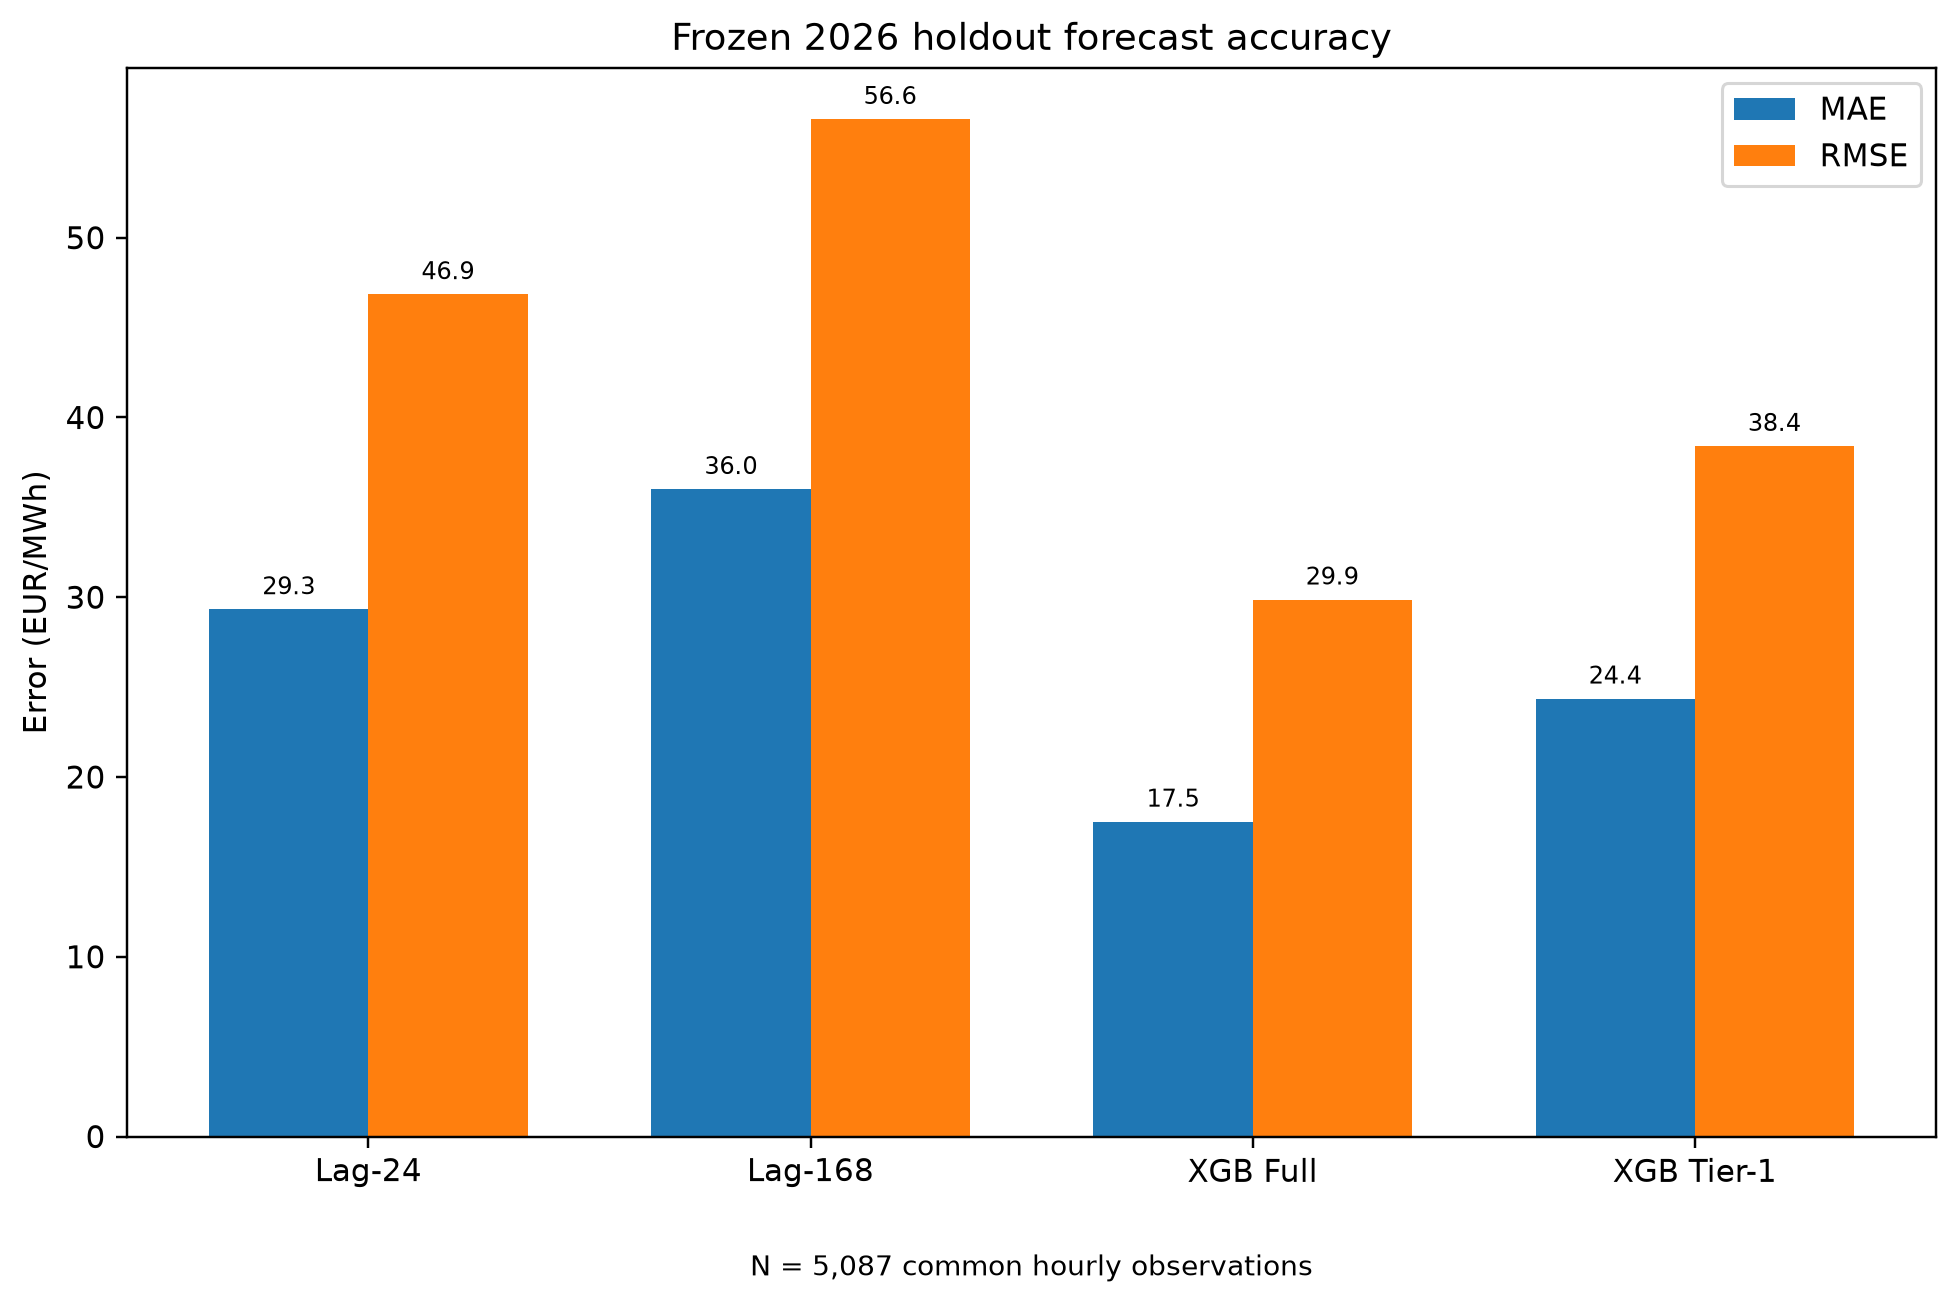
\includegraphics[width=0.92\linewidth]{figures/fig7_holdout_forecast_accuracy.png}
\caption{Point-forecast accuracy in the frozen 2026 holdout (\(N=5{,}087\) common hourly observations). Full XGBoost has the lowest MAE and RMSE, while Tier-1 XGBoost remains more accurate than both naive benchmarks.}
\label{fig:holdout_accuracy}
\end{figure}

Table~\ref{tab:holdout_forecasts} and Figure~\ref{fig:holdout_accuracy} show the same ranking. Full XGBoost reduces MAE by approximately 40.3\% relative to lag-24 and 51.4\% relative to lag-168. Tier-1 XGBoost also improves upon lag-24, with an MAE approximately 16.9\% lower, but remains materially weaker than Full.

\subsection{Primary economic results}

\begin{table}[htbp]
\centering
\caption{Frozen holdout strategy results at eta=0.85 and c=€10.}
\label{tab:holdout_strategy}
\begin{adjustbox}{max width=\textwidth}
\begin{tabular}{lrrrrr}
\toprule
Strategy & Trading days & Net P\&L & Profitable days & Hit rate & Worst day \\
\midrule
S0 & 0 & 0.00 & 0.0\% & -- & 0.00 \\
S1 & 208 & 18,564.42 & 84.0\% & 85.6\% & -67.28 \\
S2 & 210 & \textbf{20,002.02} & \textbf{91.0\%} & 91.9\% & -17.55 \\
S3 & 160 & 19,130.01 & 75.0\% & \textbf{99.4\%} & \textbf{-0.83} \\
S4 & 205 & 19,218.41 & 86.8\% & 89.8\% & -31.14 \\
S5 & 117 & 14,721.23 & 54.7\% & 99.1\% & -5.98 \\
\bottomrule
\end{tabular}
\end{adjustbox}
\end{table}

\begin{figure}[htbp]
\centering
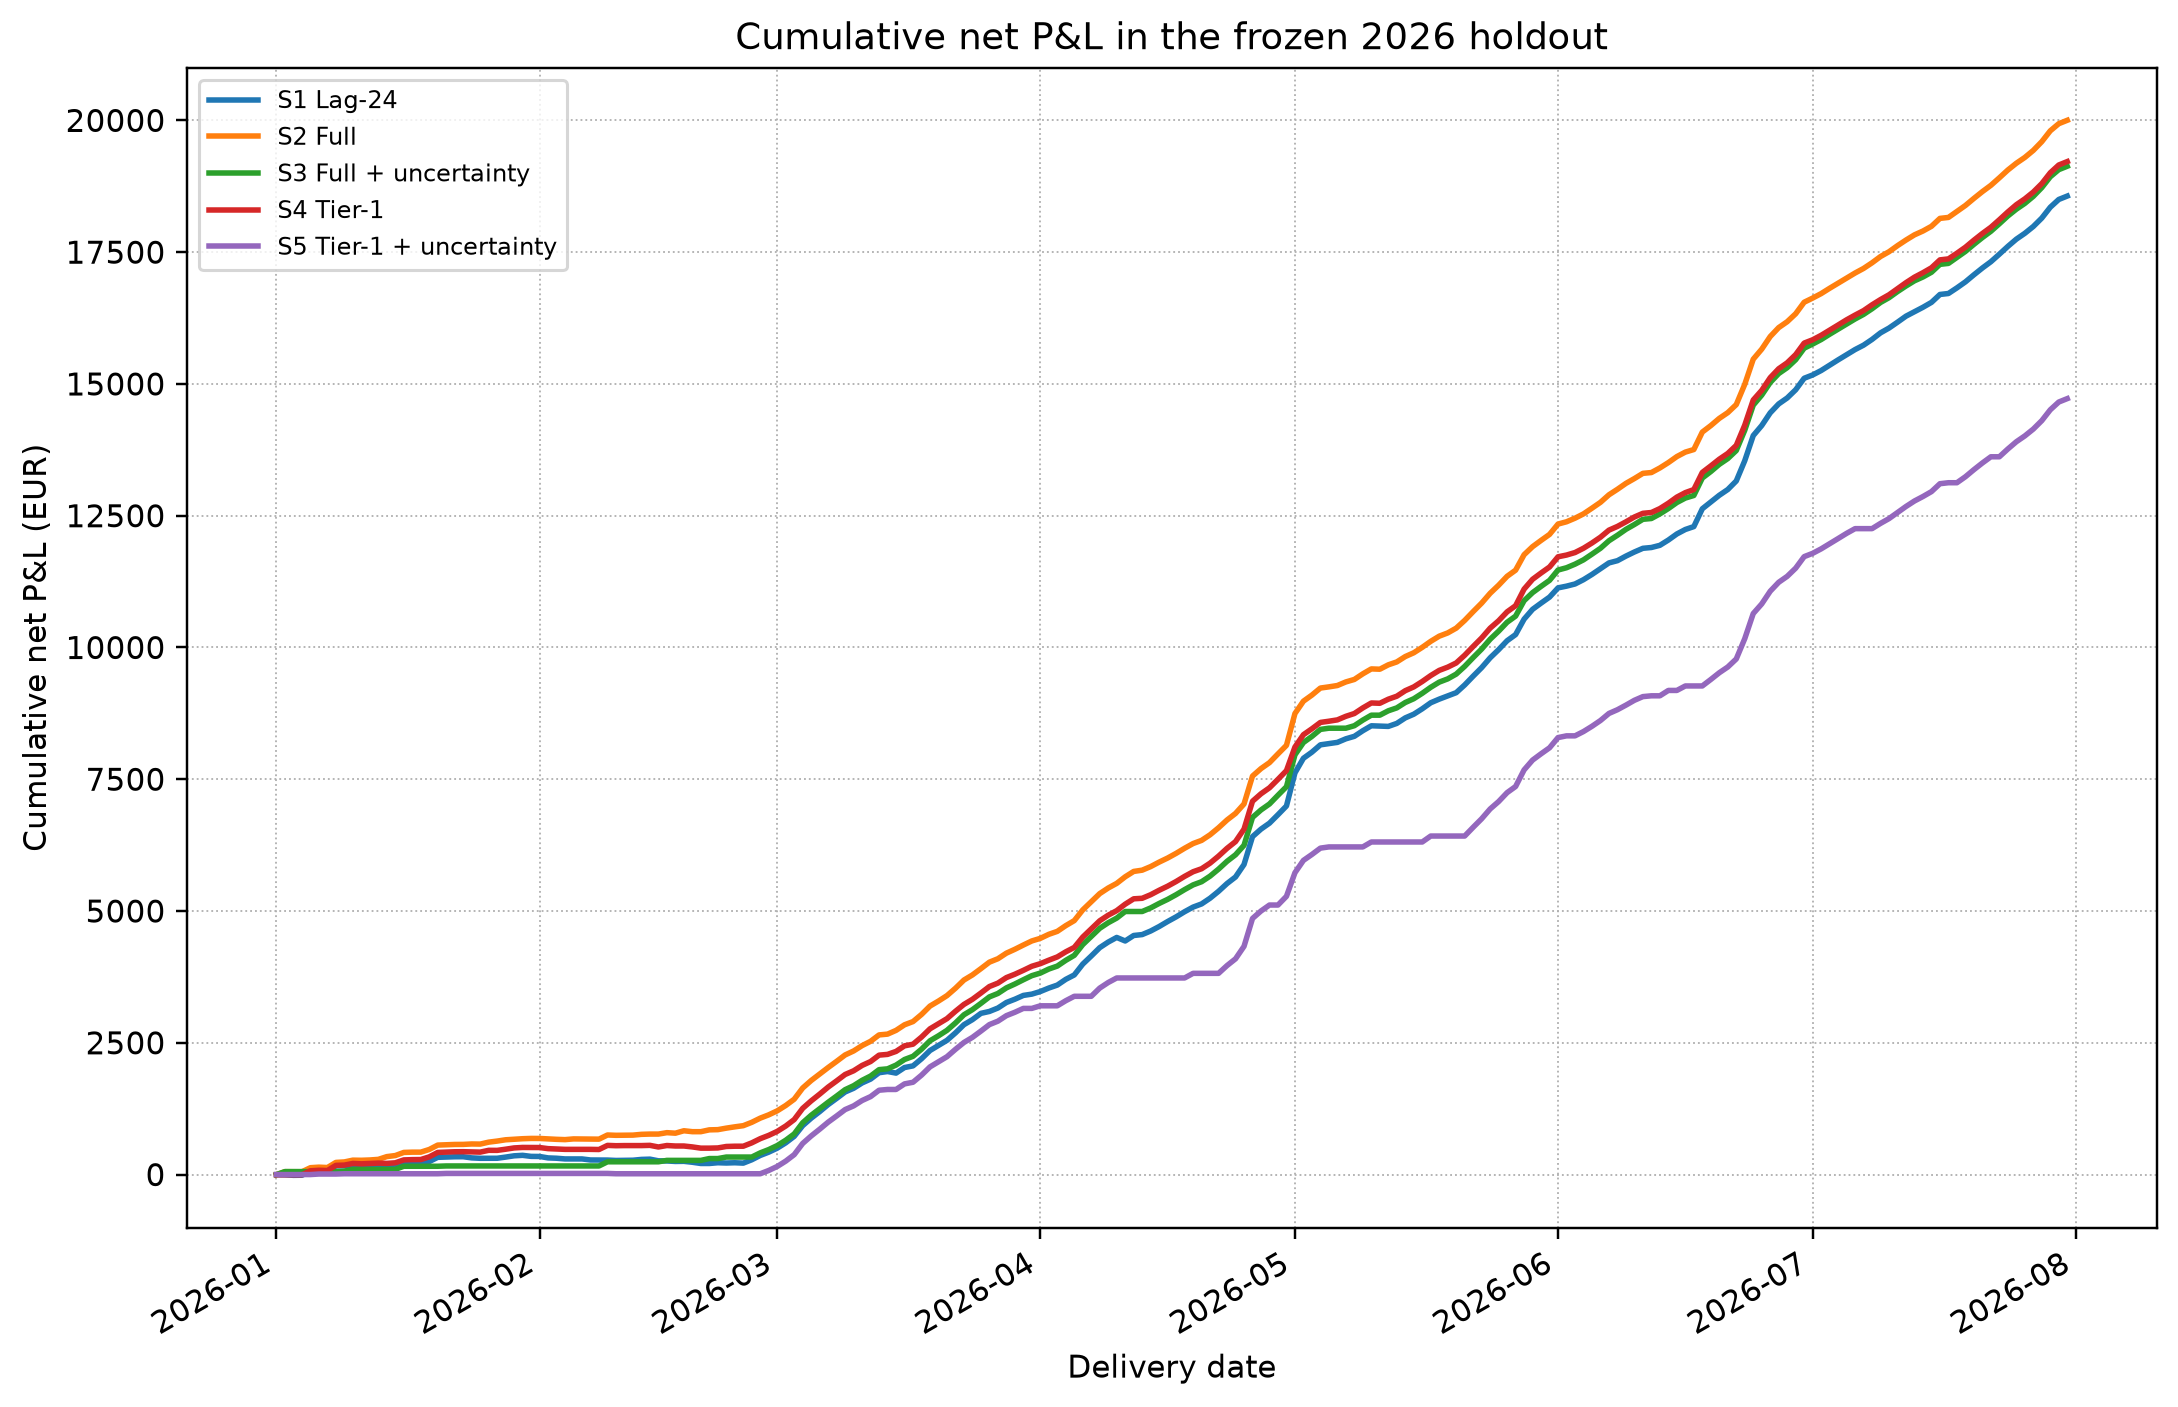
\includegraphics[width=\linewidth]{figures/fig8_holdout_cumulative_pnl.png}
\caption{Cumulative net P\&L over the 212-day frozen 2026 holdout. The curves are constructed directly from the preserved daily strategy results.}
\label{fig:cumulative_pnl}
\end{figure}

The primary contrast is
\[
\Delta_{forecast}=S2-S1=€1,437.60.
\]
Table~\ref{tab:holdout_strategy} summarizes the primary strategy outcomes, while Figure~\ref{fig:cumulative_pnl} shows their cumulative paths. The Full XGBoost point strategy earns approximately 7.7\% more cumulative net P\&L than the lag-24 strategy under the primary assumptions.

\subsection{Pre-specified nine-cell sign-consistency test}

\begin{table}[htbp]
\centering
\caption{Frozen holdout \(S2-S1\) sensitivity grid (EUR).}
\label{tab:holdout_grid}
\begin{adjustbox}{max width=\textwidth}
\begin{tabular}{rrrr}
\toprule
\(\eta_{rt}\) & \(c=5\) & \(c=10\) & \(c=15\) \\
\midrule
0.70 & 1,204.42 & 1,050.05 & 1,050.96 \\
0.85 & 1,386.14 & \textbf{1,437.60} & 1,364.73 \\
0.92 & 1,439.21 & 1,432.42 & 1,449.81 \\
\bottomrule
\end{tabular}
\end{adjustbox}
\end{table}

\begin{figure}[htbp]
\centering
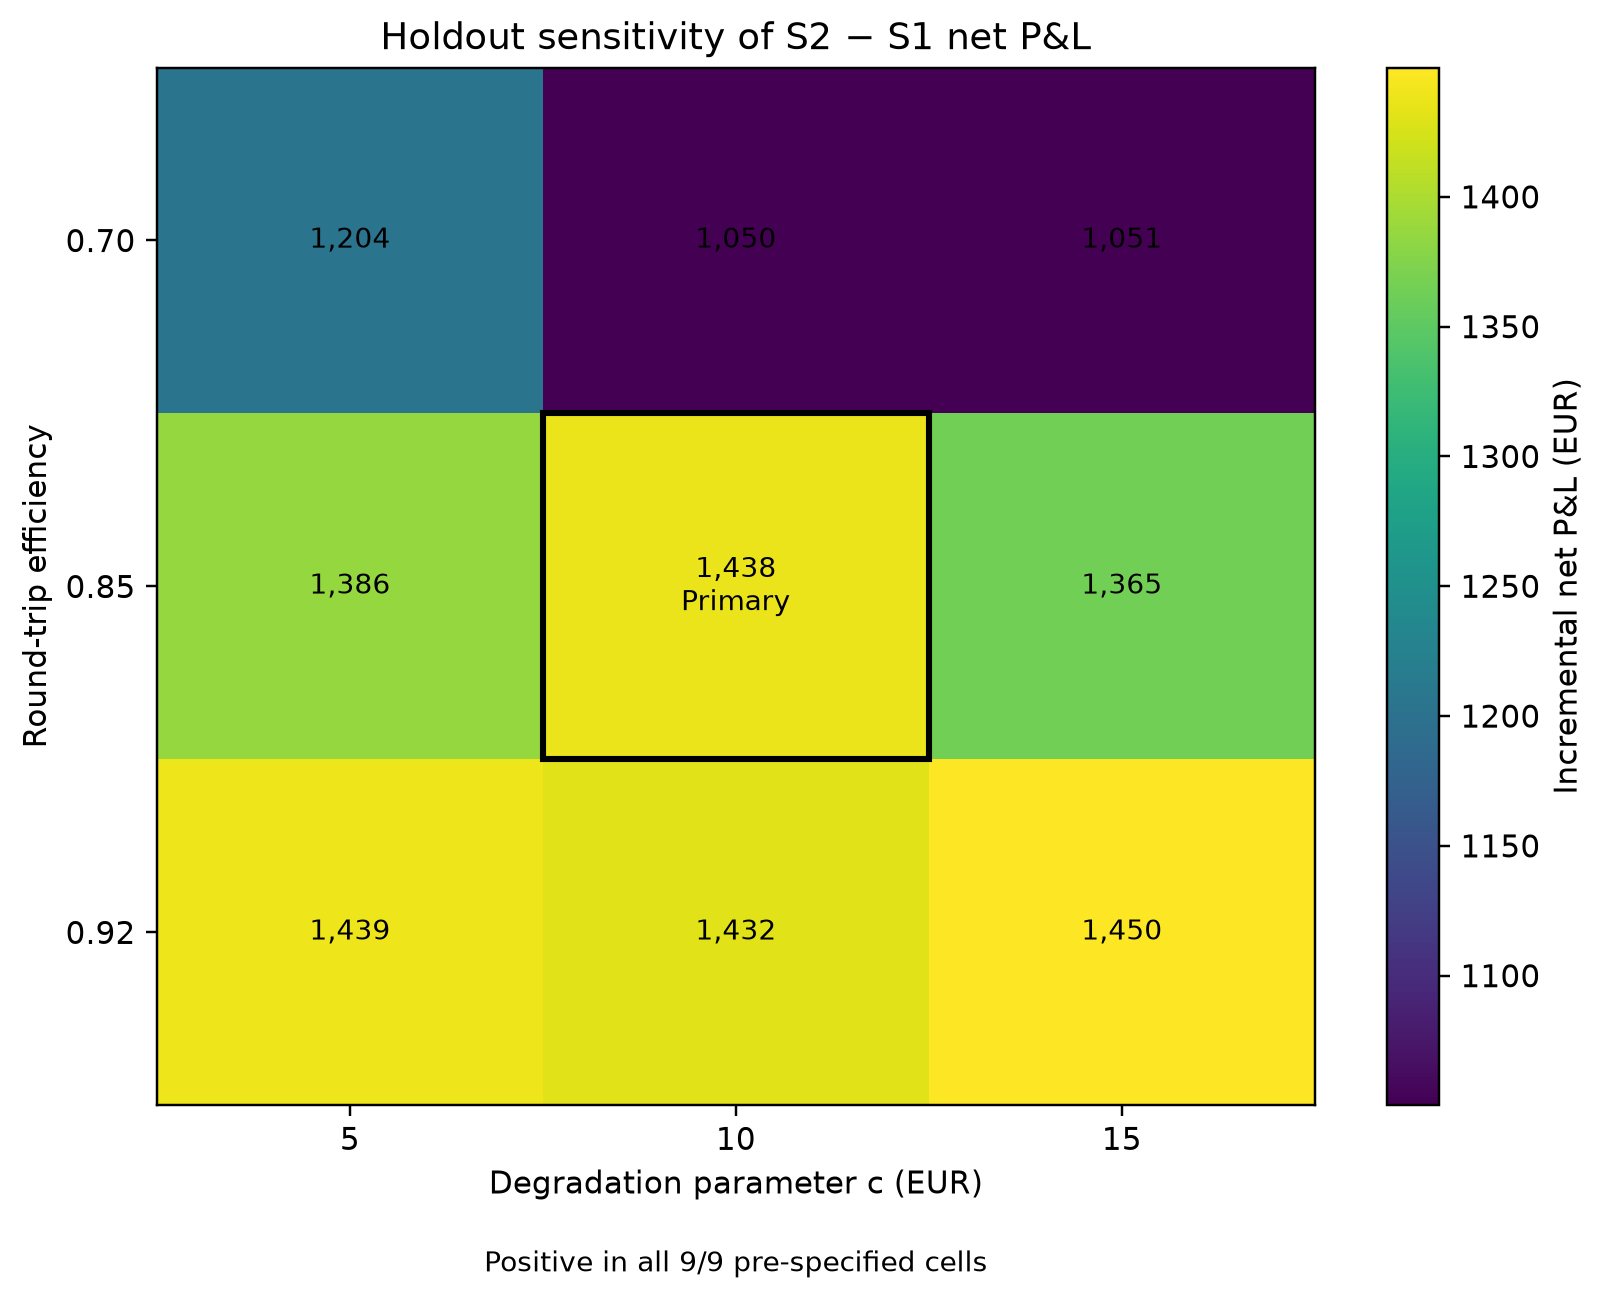
\includegraphics[width=0.88\linewidth]{figures/fig9_holdout_sensitivity_heatmap.png}
\caption{Sensitivity of the holdout forecast-value contrast \(S2-S1\) across the pre-specified efficiency and degradation-cost grid. Every cell is positive; the outlined cell is the primary setting.}
\label{fig:sensitivity_heatmap}
\end{figure}

Table~\ref{tab:holdout_grid} and Figure~\ref{fig:sensitivity_heatmap} show that the contrast is positive in all nine cells. Under the mechanical rule specified before holdout exposure, the primary forecast-value result therefore satisfies the pre-specified sign-consistency criterion. The nine cells are related sensitivity scenarios rather than independent statistical confirmations, and the criterion applies specifically to S2 over S1 under the frozen stylized contract.

\subsection{Uncertainty filtering}

The Full uncertainty-aware strategy earns €19,130.01 compared with €20,002.02 for S2, so
\[
\Delta_{uncertainty}=-€872.01.
\]

Consistent with the algebraic threshold identity in Section~\ref{sec:methods}, S2 and S3 both abstain on two days, S2 trades while S3 abstains on 50 days, and both trade on 160 days. Whenever both trade, the pair must be identical because the day-level threshold shifts every candidate pair score by the same amount; likewise, S3 cannot trade when S2 abstains. These are mechanical consequences of the frozen uncertainty construction rather than empirical discoveries.

The substantive empirical result is therefore the value of the additional abstention. The filter forgoes €952.46 of profitable opportunities and avoids €80.44 of losses, reconciling to the reported aggregate gap up to rounding.

The reduction in aggregate profit is accompanied by substantial downside improvement. The hit rate rises from 91.9\% to 99.4\%, the worst day improves from -€17.55 to -€0.83, and maximum drawdown improves from approximately -€22.61 to -€0.83.

\subsection{Tier-1 robustness}

At the primary parameters,
\[
S4=€19,218.41,
\]
giving
\[
\Delta_{Tier1}=S4-S2=-€783.61.
\]
The Tier-1 contrast is negative in all nine sensitivity cells.

The Tier-1 point estimate also exceeds lag-24:
\[
S4-S1=€653.99.
\]
This comparison was not one of the four pre-specified contrasts and is therefore reported descriptively rather than as a confirmatory economic result. In forecast accuracy, by contrast, Tier-1 materially improves on lag-24 while remaining weaker than Full.

Applying the uncertainty filter to Tier-1 produces S5, which trades on only 117 days with a 99.1\% hit rate and earns €14,721.23. It forgoes €4,654.82 of profitable outcomes while avoiding only €157.64 of losses relative to S4.

\subsection{Oracle value capture}

The ex-post oracle earns €21,243.10. The corresponding value-capture ratios are 87.4\% for S1, 94.2\% for S2, 90.1\% for S3, 90.5\% for S4 and 69.3\% for S5.

S2 therefore captures 94.2\% of the value available to the simplified perfect-hindsight oracle under the same one-cycle constraint. This ratio is a diagnostic property of the research contract, not an estimate of the fraction of real-world battery value captured.

\subsection{Tail-risk evidence}

\begin{table}[htbp]
\centering
\caption{Frozen holdout empirical daily-loss VaR and Expected Shortfall.}
\label{tab:holdout_tailrisk}
\begin{adjustbox}{max width=\textwidth}
\begin{tabular}{lrrrr}
\toprule
Strategy & VaR 95\% & ES 95\% & VaR 99\% & ES 99\% \\
\midrule
S1 & 9.72 & 26.16 & 29.64 & 48.31 \\
S2 & 2.07 & 7.07 & 8.35 & 13.45 \\
S3 & 0.00 & \textbf{0.08} & 0.00 & \textbf{0.39} \\
S4 & 5.09 & 13.02 & 20.60 & 26.82 \\
S5 & 0.00 & 0.56 & 0.00 & 2.82 \\
\bottomrule
\end{tabular}
\end{adjustbox}
\end{table}

Table~\ref{tab:holdout_tailrisk} shows that the holdout sample is too small for precise tail estimation. The 95\% tail contains only 10.6 effective observations and the 99\% tail 2.12. All holdout VaR and ES estimates are therefore flagged as low precision and used descriptively only.

\subsection{Stress-price days and concentration}

The holdout contains 69 negative-price days, 47 days with a price above €200/MWh and three days above €500/MWh. On negative-price days,
\[
\Delta_{forecast}=€153.01,
\]
while on the remaining days it is €1,284.58. On days above €200/MWh, the contrast remains positive at €262.60. The three days above €500/MWh yield identical cumulative P\&L across active strategies, so no separate inference is drawn from that very small subgroup.

S2's profits are not dominated by one extreme day: the top 1\%, 5\% and 10\% of holdout days account for 8.0\%, 18.6\% and 28.4\% of total S2 net P\&L, respectively.

\subsection{Post-hoc robustness analyses}
\label{sec:posthoc_results}

The following analyses were introduced only after exposure to the 2026 holdout and therefore do not alter the frozen primary result.

\paragraph{Stronger simple economic benchmarks.}
To compare XGBoost with simple rules that exploit recurring intraday structure, a weekday-aware naive benchmark and a trailing seven-day hourly mean profile were evaluated post hoc. The trailing-profile rule requires seven completed prior holdout days, so Table~\ref{tab:posthoc_benchmarks} uses the common 205-day sample from 8 January through 31 July 2026.

\begin{table}[htbp]
\centering
\caption{Post-hoc simple-benchmark comparison on the common 205-day sample.}
\label{tab:posthoc_benchmarks}
\begin{adjustbox}{max width=\textwidth}
\begin{tabular}{lrrrr}
\toprule
Strategy & MAE & RMSE & Net P\&L & Oracle share \\
\midrule
Lag-24 & 29.06 & 46.84 & 18,495.13 & 87.8\% \\
Weekday-aware naive & 29.89 & 47.77 & 18,372.81 & 87.2\% \\
Trailing 7-day mean profile & 29.28 & 43.59 & 19,630.98 & 93.2\% \\
XGBoost Tier-1 & 24.25 & 38.49 & 19,142.04 & 90.9\% \\
XGBoost Full & \textbf{17.51} & \textbf{30.06} & \textbf{19,869.02} & \textbf{94.3\%} \\
\bottomrule
\end{tabular}
\end{adjustbox}
\end{table}

Full XGBoost remains the most accurate model by a wide margin on this common sample, but the economic comparison is considerably tighter. Its net P\&L exceeds the trailing-profile rule by only €238.04. Tier-1 trails the trailing profile by €488.94. This shows that much of the economic value can be captured by a simple rule that learns the recurring hourly price shape, even though that rule has substantially worse point-forecast MAE than Full XGBoost.

\paragraph{Paired daily inference.}
Table~\ref{tab:posthoc_bootstrap} reports seven-day moving-block bootstrap intervals for selected daily P\&L contrasts. These intervals are supplementary and were not part of the frozen success criterion.

\begin{table}[htbp]
\centering
\caption{Post-hoc paired daily P\&L contrasts with 7-day moving-block bootstrap 95\% intervals.}
\label{tab:posthoc_bootstrap}
\begin{adjustbox}{max width=\textwidth}
\begin{tabular}{lrrrrr}
\toprule
Contrast & Days & Total difference & 95\% interval & Wins & Losses \\
\midrule
S2--S1 & 212 & 1,437.60 & [752.08, 2,140.98] & 95 & 63 \\
S3--S2 & 212 & -872.01 & [-1,459.21, -359.39] & 16 & 34 \\
S4--S2 & 212 & -783.61 & [-1,267.64, -348.12] & 49 & 97 \\
S5--S3 & 212 & -4,408.77 & [-6,189.90, -2,741.33] & 29 & 91 \\
S2--Trailing 7-day & 205 & 238.04 & [-110.21, 573.81] & 84 & 57 \\
\bottomrule
\end{tabular}
\end{adjustbox}
\end{table}

The frozen S2--S1 contrast remains positive under this supplementary paired analysis. By contrast, the Full XGBoost advantage over the post-hoc trailing-profile rule is much smaller and its block-bootstrap interval includes zero. The monthly S2--S1 decomposition is also uneven: January, February and March contribute €340.52, €367.45 and €300.87 respectively; April--June contribute €433.70 in total; July is approximately flat at -€4.94.

\paragraph{Holdout interval calibration.}
Table~\ref{tab:posthoc_calibration} summarizes post-hoc calibration of the nominal central 80\% intervals.

\begin{table}[htbp]
\centering
\caption{Post-hoc holdout calibration of the nominal central 80\% intervals.}
\label{tab:posthoc_calibration}
\begin{adjustbox}{max width=\textwidth}
\begin{tabular}{lrrrrr}
\toprule
Information set & Coverage & Lower miss & Upper miss & Mean width & Winkler score \\
\midrule
Full & 77.1\% & 9.7\% & 13.2\% & 45.12 & 89.25 \\
Tier-1 & 77.7\% & 11.3\% & 11.0\% & 71.72 & 135.31 \\
\bottomrule
\end{tabular}
\end{adjustbox}
\end{table}

Overall coverage is moderately below the nominal 80\% target for both information sets. Tier-1 achieves similar coverage only with intervals about 59\% wider than Full. Calibration is not stable over time: Full monthly coverage ranges from 69.7\% in March to 88.3\% in May, while Tier-1 ranges from 56.5\% in March to 92.2\% in May. Exploratory local-hour diagnostics also show lower Full coverage around several midday and evening hours, consistent with residual heteroskedasticity that is obscured by the pooled-hour residual construction.

\subsection{Holdout summary}

The first-look 2026 evidence supports the primary forecast-value result. Full XGBoost retains a large accuracy advantage, and the pre-specified economic contrast \(S2-S1\) is positive at the primary setting and in all nine sensitivity cells. Tier-1 has a higher economic point estimate than lag-24, but that non-pre-specified comparison is descriptive. The uncertainty-aware rule operates as an additional day-varying abstention threshold and trades aggregate profit for substantially greater selectivity and downside protection.

\section{Discussion}
\label{sec:discussion}

\subsection{Forecast accuracy survived the holdout, but economic value was not proportional to it}

The Full XGBoost pipeline generalized beyond development. Its holdout MAE is approximately 40\% below lag-24, and its economic advantage over the lag strategy remains positive in every pre-specified efficiency--cost cell. The contribution is not that a nonlinear model beat a naive benchmark. Such comparisons are common in electricity-price forecasting \citep{lago2021}. The stronger evidence is that the advantage was carried through a frozen downstream decision rule and remained positive in a separate first-look period.

The magnitude of the statistical and economic improvements differs considerably. A roughly 40\% MAE reduction produces only about a 7.7\% increase in cumulative net P\&L at the primary economic setting. This difference is consistent with established evidence. \citet{kathziel2018} show that forecast quality can translate into economic gains, while \citet{maciejowska2026} demonstrate in a closely related German/DE-LU storage setting that MAE and RMSE are only weakly associated with BESS profit. Our holdout adds complementary evidence: a large statistical improvement can survive economically, but its economic magnitude is decision-specific and much smaller than the statistical percentage improvement.

This matters for how forecasting studies should describe improved models. Statistical forecast rankings remain necessary, but they are insufficient whenever the forecast is intended to support an operational decision. Economic evaluation should be treated as a separate objective rather than an automatic consequence of lower MAE.

\subsection{Information timing is part of model validity}

The Full/Tier-1 comparison reveals a second central result. Renewable-derived variables materially improve both predictive and economic performance. Full XGBoost beats Tier-1 on the 2026 holdout, and the Full point strategy earns more in every economic sensitivity cell.

It would be tempting to interpret this simply as evidence that additional renewable fundamentals improve forecasting. That conclusion is only partly justified. Prior literature already supports the predictive value of renewable and weather information \citep{ziel2015,kathziel2018,sgarlato2023}. The unresolved issue here is whether the exact historical ENTSO-E renewable forecast values used by the Full model were publicly available at 11:45 D-1.

The evidence boundary is concrete. The regulatory load-forecast deadline is compatible with the cutoff, while the wind/solar deadline is later \citep{eureg543}. The historical interface does not preserve the complete vintage history needed to determine whether an earlier renewable forecast happened to exist for each day. Therefore the Full model's edge is real in the stored historical dataset, but its strict point-in-time reproducibility remains unproven.

Tier-1 is informative precisely because it prevents this limitation from becoming binary. The robust conclusion is not that the Full result is invalid, and not that timing does not matter. Instead, part of the advantage survives under the more defensible Tier-1 information set: Tier-1 XGBoost still reduces MAE relative to lag-24 and produces higher net P\&L. The additional Full advantage is economically meaningful, but its real-time interpretation should remain conditional on establishing the appropriate forecast vintage.

This suggests a broader methodological lesson. In public-data forecasting, information availability should be treated as a property of the versioned observation at the forecast origin, not simply as a property of the variable name.

\subsection{Uncertainty improved selectivity rather than total profit}

The uncertainty result resists a one-dimensional interpretation. The 60-day residual method was selected statistically through an interval-score rule. In the economic layer, however, adding that uncertainty information reduces cumulative P\&L in both development and holdout.

This does not mean the uncertainty layer failed. It changed a different dimension of performance. In the holdout, S3 raises the trade hit rate to 99.4\%, improves the worst day to only -€0.83, and nearly eliminates measured drawdown under the stylized contract. Mechanically, it does this by abstaining. When S2 and S3 both trade, they always choose the same pair. The uncertainty filter therefore does not discover different intraday extrema; it refuses marginal opportunities that the point forecast would take.

That behavior aligns closely with the distinction emphasized by \citet{nitka2023}: a better probabilistic forecast or scoring rule need not imply greater realized profit under a downstream decision. It also complements positive evidence from regularized probabilistic methods such as \citet{uniejewskiweron2021} and distributional approaches such as \citet{marcjasz2023}. The economic effect of uncertainty is not universal; it depends on how the distribution enters the decision rule.

Our decomposition makes the mechanism transparent. S3 forgoes €952.46 of profitable holdout opportunities while avoiding only €80.44 of losses. The value of the filter is therefore primarily downside control, not higher expected profit.

This distinction prevents two opposite overstatements. It would be wrong to conclude that probabilistic information is economically useless merely because cumulative P\&L falls. It would also be wrong to describe the filter as economically superior without specifying the objective. An operator maximizing aggregate profit would prefer S2 under the tested contract; an operator placing greater weight on avoiding losing trades might value S3 differently.

\subsection{Economic robustness and what the nine-cell result shows}

The 9/9 holdout confirmation is the strongest preregistered economic result in the study. It reduces dependence on one arbitrary choice of round-trip efficiency or degradation cost. The forecast-value contrast remains positive under all nine pre-specified combinations, including lower efficiency and higher degradation cost.

However, this grid is not a universal robustness proof. It varies two economically important assumptions while holding several others fixed. Market transaction cost is zero, market impact is absent, one cycle per day is allowed, and there is no inter-day state-of-charge constraint. As \citet{serafin2025} show, operating costs can change model rankings, while \citet{veenstra2025} emphasize that endogenous prices can matter as battery participation grows. The present sensitivity analysis should therefore be read as robustness within a clearly defined stylized contract, not as a complete commercial battery assessment.

The oracle comparison reinforces the same point. S2 captures 94.2\% of the simplified perfect-hindsight oracle, but this is not 94.2\% of all theoretically available battery revenue. It is 94.2\% of the value available to an oracle constrained to the same single-cycle daily rule and cost convention.

\subsection{The 2025 market-design transition}

All 2026 holdout observations lie after the 15-minute SDAC transition. This makes the holdout a meaningful structural stress test of a model developed primarily on the prior hourly market regime.

The pipeline explicitly handles the transition by selecting the appropriate market product, reconstructing A03 curves, averaging post-cutover quarter-hourly prices to hourly values and including a regime indicator. Full XGBoost had already retained its advantage in the October--December 2025 regime-stress fold, and the 2026 holdout extends that evidence over a longer post-transition period.

At the same time, the study does not model 15-minute decision-making. Aggregating the new market to hourly resolution intentionally sacrifices within-hour variation. A future extension should forecast and optimize directly at 15-minute resolution once a sufficiently long post-transition history is available. That would answer a different operational question and should not be retrofitted into the present frozen experiment.

\subsection{Strength of the holdout design}

The holdout protocol does not eliminate every source of uncertainty, but it changes the evidential status of the final results. The 2026 period was structurally ingested and checked before the outcome evaluation, yet its prices were not used for model selection, uncertainty-window choice, strategy tuning or economic interpretation. The final model-fit procedure, economic contract and confirmation rule were committed before the first metric was exposed.

This is consistent with the uncontaminated chronological testing emphasized by \citet{lago2021}, but the present workflow extends it into the downstream economic layer. Not only model hyperparameters but also uncertainty windows, efficiency/cost sensitivity, strategy definitions and the success criterion were frozen.

The development history also preserves corrections rather than hiding them. Price-product selection, local delivery-day cutovers, DST-safe lags, A03 reconstruction and the delivery-day uncertainty correction were all addressed before final holdout exposure, with superseded artifacts retained as an audit trail. Reproducibility therefore includes not only the ability to rerun final code but also the ability to understand how consequential methodological errors were found and corrected.

\subsection{Limitations}

Several limitations materially constrain interpretation.

First, Tier-2 point-in-time availability remains unresolved. The Full model should not be described as a deployable 11:45 D-1 system until appropriate historical or live publication vintages are independently verified.

Second, the economic model is intentionally stylized. It assumes price-taking, one charge-discharge cycle per day, no inter-day energy carry, zero explicit exchange/clearing/brokerage cost, and no market impact. It also omits capital expenditure, financing, ancillary services and battery-health dynamics beyond the fixed throughput degradation cost.

Third, uncertainty is based on marginal empirical residual quantiles. It does not model the multivariate dependence structure of the full delivery-day price vector. Richer multivariate probabilistic post-processing could support different storage decisions, but introducing it after the holdout would constitute a new experiment rather than an extension of the frozen result.

Fourth, the holdout covers only seven months and one post-transition market regime. Tail-risk precision is particularly weak: 99\% VaR/ES rests on approximately two effective observations. Those values are descriptive and should not be treated as stable extreme-risk estimates.

Fifth, formal statistical-significance testing was not part of the pre-registered confirmation rule. Predictive-comparison tools such as Diebold--Mariano or conditional predictive-ability tests \citep{diebold1995,giacomini2006} could be reported as supplementary post-hoc inference, but they should remain clearly separated from the frozen primary result.

\subsection{Implications for forecast-to-decision research}

Three broader implications follow. First, point-in-time data provenance deserves the same status as model architecture. A sophisticated model estimated on uncertain vintages can provide a less defensible result than a simpler model estimated on a clearly admissible information set.

Second, uncertainty should be evaluated according to the decision objective it changes. Statistical calibration, cumulative profit, trade hit rate and downside risk are distinct outcomes and need not improve together.

Third, final economic evaluation should be protected from the same adaptive overfitting that forecasting researchers recognize at the model-selection stage. Once thresholds, costs, filters and sensitivity grids are chosen after viewing test profits, the economic backtest itself becomes a tuning exercise. Freezing the full forecast-to-decision contract before outcome exposure provides a practical way to reduce this risk.

\section{Conclusion}
\label{sec:conclusion}

This study asked whether a day-ahead electricity-price forecasting advantage survives explicit information constraints and translates into economic value when forecasting, uncertainty and trading rules are frozen before final evaluation.

Using public ENTSO-E data for the Germany--Luxembourg market, models were developed on 2019--2025 data and January--July 2026 was reserved for a first-look holdout. The final design distinguished a Full information set from a Tier-1 robustness set, used chronological model selection, constructed uncertainty from delivery-day-safe out-of-sample residuals, and mapped forecasts into a pre-specified single-cycle storage decision rule.

The primary result survives the holdout. Full XGBoost attains an MAE of €17.51/MWh compared with €29.33/MWh for lag-24. Under the primary economic assumptions, the Full point strategy earns €20,002.02, or €1,437.60 more than the lag-24 strategy. The forecast-value contrast remains positive in all nine pre-specified efficiency--cost cells, satisfying the mechanical holdout confirmation criterion.

The secondary results qualify that conclusion in useful ways. Tier-1 XGBoost remains more accurate and economically valuable than lag-24, but it is materially weaker than Full, showing that the unresolved renewable-vintage issue is economically consequential. The uncertainty-aware Full strategy sacrifices €872.01 of cumulative net P\&L but raises the trade hit rate to 99.4\% and reduces the worst daily outcome to -€0.83. Uncertainty therefore acts as a conservative abstention mechanism rather than a profit-maximizing layer under the tested rule.

The paper's contribution is not a new forecasting algorithm and not the observation that forecast accuracy and economic value can diverge. Instead, it demonstrates a reproducible forecast-to-decision workflow in which information timing, model selection, uncertainty construction, economic assumptions and the final evaluation are treated as one research design.

The principal unresolved issue is now clear. Before the Full model can be interpreted as a genuinely deployable 11:45 D-1 system, historical or live renewable forecast vintages must be verified at that exact decision origin. Future work should also move directly to 15-minute forecasts and decisions, represent multivariate price-path uncertainty, include more complete battery and market-access costs, and accumulate a longer post-transition holdout for more credible tail-risk inference.

The broader lesson is that useful forecast evaluation begins after the forecast is produced. A forecast is operationally valuable only if the information used was genuinely available, the decision rule was specified before outcomes were known, and the claimed economic gain survives assumptions that matter to the decision.


\section*{Data and code availability}
The complete research pipeline, frozen protocols, model artifacts, development outputs and 2026 holdout outputs are available at \url{https://github.com/Jonathanerrils/european-power-forecast-trade}. The repository preserves superseded development artifacts where methodological corrections occurred so that the research audit trail remains visible. ENTSO-E market data are subject to the source platform's terms of use.

\section*{Declaration of competing interest}
The author declares no competing interests.

\section*{Funding}
This research received no external funding.

\section*{Declaration of generative AI and AI-assisted technologies in the writing process}
During preparation of this manuscript, the author used ChatGPT to assist with language editing, manuscript organization and LaTeX preparation. The underlying research design, code, data analysis, interpretation and final verification remain the responsibility of the author. This statement should be adapted to the policy of the target journal at submission.

\section*{Acknowledgements}
To be added before submission.

\bibliographystyle{elsarticle-harv}
\bibliography{references}

\appendix
\section{Frozen research provenance}
\label{app:provenance}
The pre-holdout protocol was frozen in the repository at commit
\texttt{a2d1f9a79022ca1e2731d52803061825038c69f5}. The final Full and Tier-1 model fit was frozen at commit
\texttt{54a7c2e77122134eca31a09798cc1614df1c634c}. The accepted corrected development lineage is identified by
\texttt{xgboost\_v1\_a03fix}, \texttt{uncertainty\_selected\_v2\_dayorigin},
\texttt{strategy\_report\_v2\_dayorigin} and \texttt{strategy\_tailrisk\_v2\_dayorigin}.
The preserved holdout artifacts are \texttt{holdout\_v1},
\texttt{holdout\_report\_v1}, \texttt{holdout\_sensitivity\_v1} and
\texttt{holdout\_tailrisk\_v1}.

\end{document}
